\documentclass[12pt, handout]{beamer}
\usetheme{Warsaw}
\usepackage{multimedia}
\usepackage{graphicx}
\usepackage{url}
\usepackage[utf8]{inputenc}

\AtBeginSection[]
{
	\begin{frame}
		\frametitle{Table of Contents}
		\tableofcontents[currentsection]
	\end{frame}
}

\title{Master's thesis}
\subtitle{Simulation of complex actuators}
\author{Hubert Woszczyk}
\institute{Univerity of Liège}
\date{Academic year 2015-2016}

\begin{document}
	
\frame{\titlepage}

\section{Introduction}
\frame{\frametitle{Context \& Motivation}
	\centering
	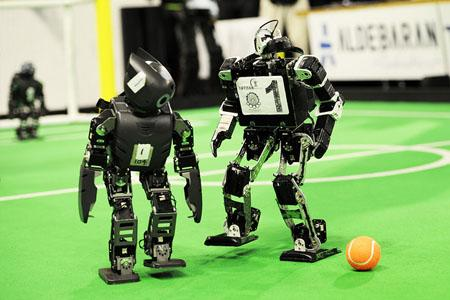
\includegraphics[width=0.7\textwidth]{images/intro_roboSoccer}
}

\frame{\frametitle{Subject of work}
	Required features:
	\begin{itemize}
		\item realistic physics simulation
		\item ability to control the simulation from outside
		\item the model of the robot should receive instructions at a relatively high frequency and be able to interpret the same instructions that the real robot will
	\end{itemize}
}

\section{Choices}
\frame{\frametitle{Choices}
	\centering
	\includegraphics[width=\textwidth]{images/overview}
}


\section{Modelling}
\frame{\frametitle{Modelling}

}

\section{Simulation}
\frame{\frametitle{Simulation modus operandi}

}

\section{Applications}
\frame{\frametitle{Applications (1/2)}
\centering
\movie[label=show3,width=0.8\textwidth, poster]{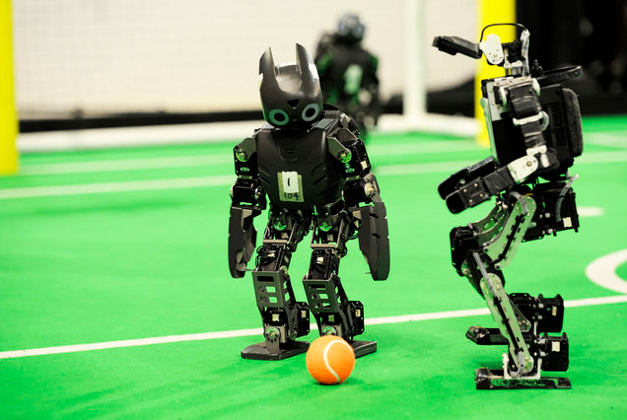
\includegraphics[width=0.8\textwidth]{images/intro_ks}}{prone.avi}
}

\frame{\frametitle{Applications (2/2)}
\centering
\movie[label=show3,width=0.8\textwidth, poster]{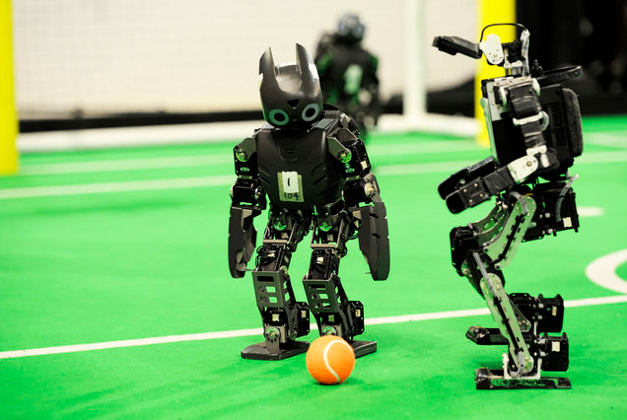
\includegraphics[width=0.8\textwidth]{images/intro_ks}}{prone.avi}
}

\end{document}
